\section{Agenti e razionalità}
Il campo dell'\textbf{intelligenza artificiale} ha lo scopo di comprendere e creare entità intelligenti, macchine capaci di calcolare come agire in modo
efficace e sicuro in base alla situazione presa in esame. Si tratta di una disciplina molto ampia e suddivisa in un gran numero di sottoinsiemi; alcuni
di questi, come l'apprendimento e la percezione, sono ambiti generali, mentre in altre diramazioni si applica l'AI anche per problemi specifici, come la
dimostrazione di teoremi matematici. Esistono più scuole di pensiero riguardanti la definizione formale di "intelligenza"; una prima idea, che ha
origine dalla psicologia, vede più intelligenti quelle entità capaci di rispecchiare al meglio la mente umana, ma tendenzialmente si preferisce usare
la nozione di \textbf{razionalità}, ovvero, dato un problema particolare, di compiere un'azione corretta per avvicinarsi alla sua risoluzione.\par
Le entità usate in questa disciplina si chiamano \textbf{Agenti}, i quali rappresentano un sistema capace di percepire il suo ambiente attraverso dei
\textbf{sensori} e agisce su di esso mediante \textbf{attuatori}; non dissimilmente da come una persona percepisce e interagisce con ciò che lo circonda.
In particolare, i dati percepiti dagli agenti formano una \textbf{sequenza percettiva}, ovvero lo storico di quanto da essi osservato all'interno del
loro ambiente. Il comportamento di un agente è poi descritto da una \textbf{funzione agente}, la quale mostra la corrispondenza tra una qualsiasi
sequenza percettiva e una specifica azione, ed è implementata dal \textbf{programma agente}, un algoritmo in esecuzione all'interno del sistema
fisico.\par
Potendo inserire diversi algoritmi usati come programma agente, è necessario capire in che modo determinare quando un agente è adatto al compito che gli
è richiesto di eseguire. Richiamando il precedente concetto, definiamo \textbf{agenti razionali} quei sistemi che eseguono un'azione "corretta", atta
alla risoluzione del problema, la quale è valutata in base a una \textbf{misura di prestazione}, il criterio per definire quanto efficaci siano state.
In questi termini, è auspicabile massimizzare il valore atteso da questa misura per ogni sequenza percettiva ottenibile, mostrando come la qualità di
un agente sia un problema di ottimizzazione.
\begin{figure}[h]
    \centering
    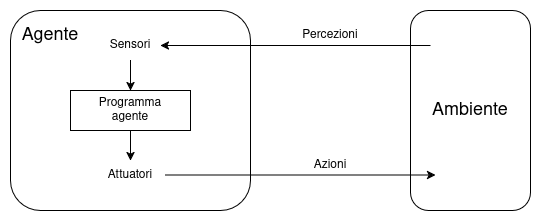
\includegraphics[width=0.8\linewidth]{Images/Agent.png}
    \caption{Struttura di un agente}    
\end{figure}

\noindent Supponiamo per esempio un ambiente composto da due stanze sporche e l'obiettivo è pulirle tutte. Si potrebbe usare il seguente programma
agente per rimuovere lo sporco: \begin{algorithm}[h]
    \caption{Reflex-Vacuum-Agent(location, status) \textbf{returns} action}
    \begin{algorithmic}[i]
         \If{status = dirty} \textbf{return} Suck
         \ElsIf{location = A} \textbf{return} Right
         \ElsIf{location = B} \textbf{return} Left
         \EndIf
    \end{algorithmic}
\end{algorithm}

\noindent Se l'unica misura di prestazione è la pulizia dell'ambiente, possiamo dire che questo agente è razionale e buono, ma se si aggiungessero
ulteriori condizioni sarà necessario rivedere l'algoritmo utilizzato. È comune, in problemi come questo, usare come misura il valore di \textbf{average
idleness}, la somma degli intervalli di tempo per i quali l'agente non visita altri stati, per poterla minimizzare e risolvere il problema il prima
possibile. In questi termini è desiderabile considerare tutti gli stati allo stesso modo, con lo scopo di ottenere valori medi i più omogenei possibile.
Ciò si traduce nel cercare di minimizzare il valore di varianza, siccome più basso sarà, tanto più omogenei saranno i valori di idleness.

%

\section{Struttura degli agenti}
Ora che abbiamo compreso le componenti che formano gli agenti razionali, è necessario fornire una visione più formale di cosa definire per poterli
progettare al meglio. Gli elementi sono dati dall'acronimo \textbf{PEAS}, ovvero: \begin{itemize}
    \item \textbf{Performance measure}: Risultato desiderato dall'agente.
    \item \textbf{Environment}: Ambiente di lavoro al quale è applicato l'agente.
    \item \textbf{Actuators}: Elementi che definiscono come l'agente può compiere azioni.
    \item \textbf{Sensors}: Elementi che definiscono come l'agente è in grado di percepire l'ambiente.
\end{itemize}

\noindent Esistono inoltre diversi tipi di ambienti con una struttura condivisa per poter definire il tipo di problema preso in esame. È di fondamentale
importanza conoscerli a fondo poiché il design degli algoritmi si baserà in gran parte su di essi: \begin{itemize}
    \item \textbf{Osservabile}: Lo stato del mondo è completamente visibile dall'agente.
    \item \textbf{Deterministico}: Le azioni hanno conseguenze perfettamente predicibili dall'agente.
    \item \textbf{Episodico}: Le azioni che l'agente compie impattano esclusivamente la sola istanza di lavoro corrente. Ciò non fa cambiare strategia.
    \item \textbf{Statico}: Si lavora sempre nello stesso ambiente non modificabile; solo le azioni dell'agente potranno cambiare.
    \item \textbf{Discreto}: Il problema è esprimibile con sole variabili discrete.
    \item \textbf{A singolo agente}: Il problema presenta l'utilizzo di un singolo agente.
\end{itemize}

\noindent In base al tipo di problema proposto, si tenderà a cadere in uno dei seguenti quattro tipi di agenti: \begin{itemize}
    \item \textbf{Simple-reflex}: Crea una risposta in base alla percezione corrente e le condizioni interne.
    \item \textbf{Reflex with state}: Come il precedente, ma mantiene anche uno stato interno. Comunemente utilizzato quando la conoscenza dell'ambiente
        non è sufficiente a determinare una risposta.
    \item \textbf{Goal-based}: Mantiene un obiettivo finale da raggiungere e presenterà un blocchetto di codice in più per osservare come il mondo si
        evolve in base alle proprie azioni. Richiede un environment completamente osservabile e deterministico per funzionare.
    \item \textbf{Utility-based}: Fornisce un valore di utilità a ogni stato e il suo scopo è massimizzare quanto ottenuto.
\end{itemize}

\noindent Ognuna di queste quattro categorie di agente ha la possibilità di diventare \textbf{intelligente}, per i quali è assegnato un critico il cui
compito è dire all'agente quanto bene sta performando in base alla misura di prestazione stabilita.

%

\section{Agenti Problem-solving}
Se consideriamo gli agenti goal-based, ovvero basati su obiettivi, è possibile delinearne un sottoinsieme composto da quelli capaci di \textbf{risolvere
problemi}, i quali formulano un obiettivo e un problema dato lo stato corrente, per cercare una soluzione ed eseguirla.
Le loro variabili che compongono l'ambiente vengono quindi inizializzate una sola volta, all'inizio, e sono: \begin{itemize}
    \item \textbf{seq}: Sequenza di azioni compiute dall'agente.
    \item \textbf{state}: Descrizione dello stato corrente dell'ambiente.
    \item \textbf{goal}: Obiettivo definito all'avvio.
    \item \textbf{problem}: Formulazione del problema. visto come quadrupla di stato iniziale, funzione successore, goal test e path cost.
\end{itemize}

\noindent In particolare, i problemi sono definiti da una quadrupla composta da \textbf{stato iniziale}, \textbf{funzione successore}, la quale a sua
volta è un insieme di coppie (azione, stato) $S(A) = \{\left<state_1\to state_2\right>, ...\}$, \textbf{goal test}, indicante l'obiettivo, e il
\textbf{costo del percorso}, un valore additivo dato per esempio dalla somma del costo di attraversamento degli archi in un grafo.\par
Dunque, all'avvio, quando \textit{seq} è vuota, si formulano \textit{goal} e \textit{problem} e si attua il processo di ricerca sul problema per poter
determinare la prima azione da compiere e aggiungere alla sequenza. Dopo questa prima iterazione, si riparte e l'agente aggiornerà lo stato ricevendo
una nuova percezione. Il processo continua fino al termine della ricerca. In pseudocodice: \begin{algorithm}[h]
    \caption{Simple-Problem-Solving-Agent(percept) \textbf{returns} action}
    \begin{algorithmic}[i]
        \State state $\gets$ Update-State(state, percept)
        \If{seq is empty}
            \State goal $\gets$ Formulate-Goal(state)
            \State problem $\gets$ Formulate-Problem(state, goal)
            \State seq $\gets$ Search(problem)
        \EndIf
        \State action $\gets$ First(seq)
        \State seq $\gets$ Rest(seq)
        \State \textbf{return} action
    \end{algorithmic}
\end{algorithm}

\noindent Questo è rappresentativo di un agente basato su obiettivi applicato in un ambiente deterministico e completamente osservabile, ma non sempre
è possibile conoscere tutto; in tal caso si avrebbe un problema \textbf{conformant}, dove l'agente sarebbe cieco e non avrebbe modo di capire dove si
trovi, né se sta lavorando bene.\par
Se invece i problemi non sono deterministici o parzialmente osservabili, si ha un problema di \textbf{contingenza}, nel quale le percezioni forniscono
informazioni nuove in base allo stato corrente e il problema dovrà essere risolto con un piano di contingenza.\par
Infine, se lo spazio degli stati è del tutto socnosciuto, si ha un problema di \textbf{esplorazione} e per risolverlo sarà necessario usare quello che
è conosciuto come reinforcement learning.